\section{Time-Series Clustering and Classification}

\subsection{Clustering}

Clustering groups time series by their similarity. The most similar series fall into the same cluster, while distinct clusters stay dissimilar from one another. The groups are not predefined, so this is an unsupervised learning task.

For time series, the two most common methods are partitional clustering and hierarchical clustering. \textbf{Partitional clustering} uses the K-means algorithm (or some variant) to optimize the objective function by minimizing the SSE. It is perhaps the most widely used clustering algorithm in the literature. One of its shortcomings is that the number of clusters, $K$, must be pre-specified. The distance function also plays a fundamental role, both for the quality of the results and for the efficiency. \textbf{Hierarchical clustering} starts by computing the pairwise distance between time series, using whatever distance measure the user specifies, and then merges clusters bottom-up, joining the two closest clusters at each step until a single cluster contains every data point. This approach is limited to small datasets, since its computational complexity is quadratic.

Time series clustering can be of the following types:
\begin{itemize}
    \item \textbf{Whole clustering}: the conventional type of clustering, where the goal is to assign each data object to a cluster.

    \item \textbf{Feature-based clustering}: features (or motifs, see next section) are extracted from the series, and then used to cluster.

    \item \textbf{Compression-based clustering}: compress time series and run clustering on the compressed versions.

    \item \textbf{Subsequence clustering}: clustering is performed on the subsequences extracted from a single long time series with a sliding window.
\end{itemize}

\subsection{Motif and Discord Discovery}
\begin{definition}[Motifs \& Discords]
\textbf{Motifs} are repeated patterns/subsequences within a time series. \\ \textbf{Discords} are exceptionally unusual patterns within a time series.
\end{definition}
Motif discovery is a preprocessing phase for several later analyses: mining association rules, where motifs are referred to as primitive shapes and frequent patterns; classification, which in some cases works by constructing a typical prototype (motif) for each class; and anomaly detection, whose algorithms use motifs to model typical time-series behaviour and then flag future patterns that are dissimilar.

Given a predefined motif length $m$, a brute-force approach would search all possible motifs obtainable from every comparison of subsequences of length $m$. This is clearly inefficient. The most commonly used algorithm was originally developed in bioinformatics, and is based on \textbf{random projections} and SAX, which lets it work on lower-bound discrete representations of the series.

First, an alphabet size $\alpha$, a SAX window size $w$, and a motif length $n$ are set. All approximated subsequences of length $w$ are extracted via SAX from the time series by shifting the window forward one measurement at a time, for a total of $|T| - (n - 1)$ subsequences. Then a mask is chosen at random to select only certain ``columns'' of the subsequences: if the mask $\{1,3\}$ is chosen, only the first and third symbols in the representation are considered. Collisions between masked subsequences are recorded in a \textbf{collision matrix} by incrementing the corresponding cell. The step repeats several times with different masks.

After these random perturbations, motifs show up in the collision matrix as the cells with the highest values: their indices are the positions where the motifs start in the time series. The weakness of the approach is its heavy dependence on the approximation technique: change one parameter and the outcome changes entirely, which is why we turn to the Matrix Profile.

\subsubsection{Matrix Profile}
Given a time series $T$, we first compute the pairwise distance among all the $|T| - (n - 1)$ subsequences that a sliding window of length $n$ extracts from $T$ (the window captures the shifting effect). The \textbf{Matrix Profile} (\textbf{MP}) of $T$ is then the vector that annotates the distance between each subsequence and its nearest neighbor. The index of that nearest neighbor is stored in a separate vector, the \textbf{Matrix Profile Index}, which locates the nearest neighbor in constant time. These pointers are not necessarily symmetric: if $n$ is the nearest neighbor of $m$, the nearest neighbor of $n$ need not be $m$, but may be some other subsequence. For the two smallest values in the MP, however, the pointers of the corresponding subsequences must be mutual. A valley in the matrix profile marks a region of high similarity.
\begin{definition}[Matrix Profile]
The \textbf{Matrix Profile} is a \textit{data structure} that annotates a TS and can be exploited for many purposes, such that efficient motifs discovery.
\end{definition}

\begin{figure}[h]
    \centering
    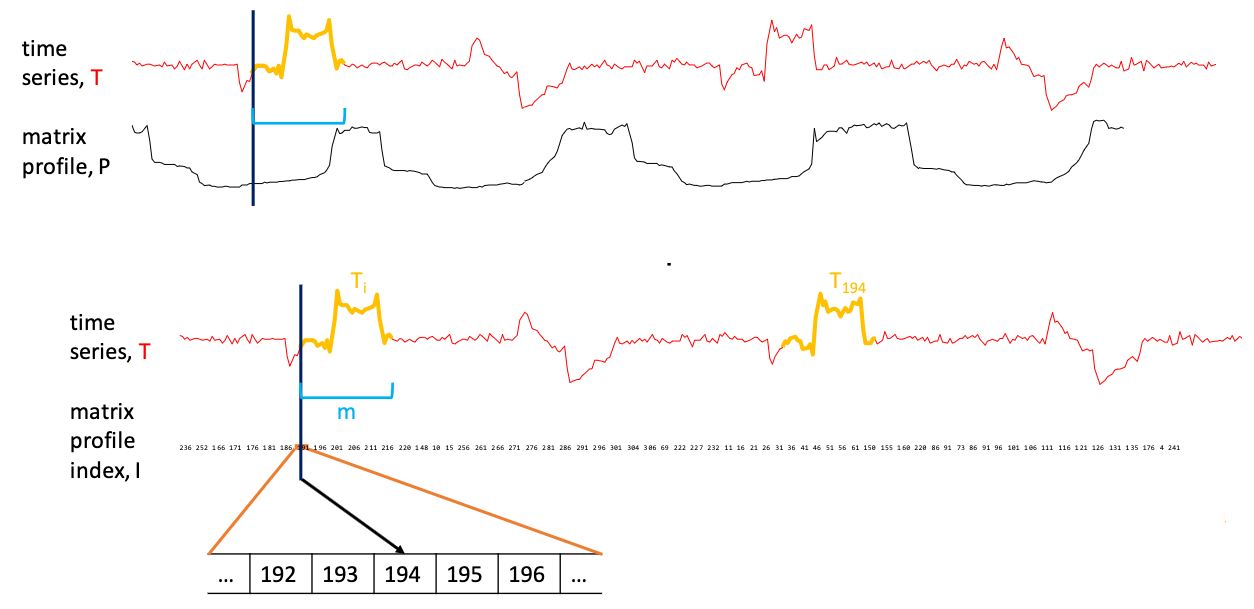
\includegraphics[width=0.9\linewidth]{img/mp_mpi.png}
    \caption{Matrix Profile (on top) and Matrix Profile Index (on the bottom).}
    \label{fig:mp-mpi}
\end{figure}

Low values in the matrix profile indicate that the corresponding subsequence has at least one similar subsequence in the data: these regions mark motifs. Regions with very high values instead mark discords, subsequences whose nearest neighbor is far away.

To compute the matrix profile of a time series $T$ for a desired subsequence length $m$, the cells of the vector are initialized to $\infty$. A random subsequence $T_i$ is then selected, and its distance to every other subsequence is stored in a separate vector; this step has complexity $O(|T| \log(|T|))$. The matrix profile is updated by taking the element-wise minimum of the two vectors, skipping the cell for $T_i$ (which on the first step keeps $\infty$). A new subsequence is selected at random and the process repeats, refreshing the matrix profile with the new minima. The algorithm stops once every subsequence has been selected. There are $|T|$ subsequences, so the total time complexity is $O(|T|^2 \log(|T|))$.

It helps to think of time-series subsequences as points in an $m$-dimensional space: very similar subsequences lie close together in denser areas, which in turn correspond to low-value regions of the MP. This data-point interpretation explains how the \textit{top-k motifs} are extracted. A parameter $R$ with $\textit{small number} > R > 1$ is chosen, and the two nearest points are found, called the \textbf{motif pair}; this pair of subsequences corresponds to the lowest pair of values in the MP. Given the distance $D_1$ between the two points, a circle of radius $D_1 * R$ is drawn around each: any point falling within either circle joins the motif, giving the top-1 motif. To find the top-2 motif, the next closest pair of points is found (excluding those already in the previous motif), at distance $D_2 > D_1$; a circle of radius $D_2 * R$ is drawn around each, and every point inside is added to the motif. With many time series, we can run K-Means first. To decide when to stop, that is, to fix the value of $k$, we either use a predefined value or the Minimum Description Length.

\begin{figure}[H]
    \centering
    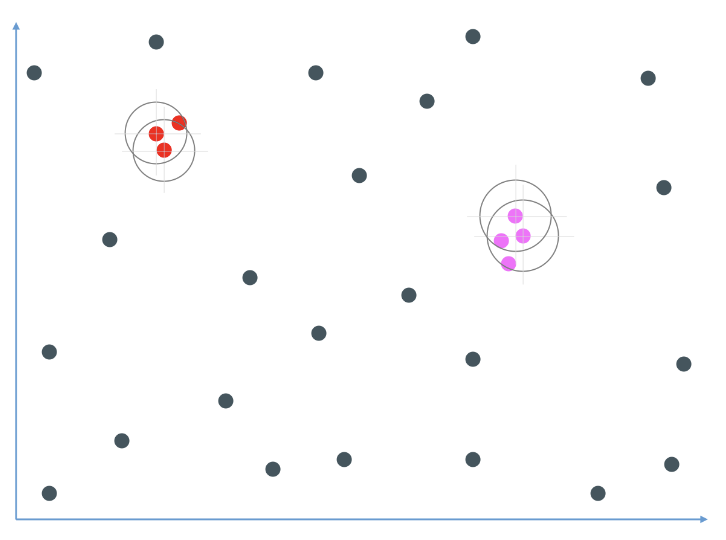
\includegraphics[width=0.35\linewidth]{img/topk_motifs.png}
    \caption{A graphical interpretation of how top k-motifs are found. The red dots are the top 1-motif, and the magenta ones are the top-2 motifs.}
    \label{fig:top-k-motifs}
\end{figure}

To find the top-k discords instead (anomaly discovery), a parameter $E$ sets how many subsequences near an anomaly are excluded, and the subsequence with the highest distance in the MP is found: this is the biggest anomaly. The $E$ subsequences closest to that anomaly are then removed together with it. As before, $k$ is either fixed to a predefined value or chosen via the MDL.

\subsection{Classification}

For a classification task we are given a set of $n$ time series, all assumed of length $m$, each series $x_i$ carrying a class label $c_i$. We thus consider a set $X$ of $n$ time series, $X:\{x_1,..,x_n\}$, each with $m$ ordered values $x_i=\{x_{i1},..,x_{im}\}$ and a class value $c_i$. The objective is to find a target function $f$ that maps every possible time series to the space of possible class values. The most widely used algorithm for time-series classification is K-NN on the raw data. It is simple and pairs well with Dynamic Time Warping (DTW), which beats Euclidean distance on many problems. It is a lazy classifier, though, so prediction is already costly, and DTW slows execution further. K-NN classification also gives little insight into the data.

An alternative is \textbf{shapelet-based classification}. Shapelets are time-series subsequences that are maximally representative of a class with respect to a given dataset of series. Once extracted, they transform the dataset into a form usable as classifier input; they also yield interpretable results and can be remarkably accurate, since they are local features, unlike most time-series classifiers that consider only global features. They tend to be faster at classification than other methods, because the prediction phase costs only $O(ml)$, where $m$ is the length of the query time series and $l$ is the length of the shapelet. DTW-based K-NN, in contrast, has time complexity $O(km^3)$, where $k$ is the number of objects in the training set.

Since shapelets are much shorter than the series they come from, we need a measure of the similarity between a subsequence and a time series. The distance between two time series $T$ and $S$, with $|S| < |T|$, is computed as:
\begin{equation*}
    \textit{SubsequenceDist}(T,S) = \min(\textit{Dist}(S,S')) \ \forall S' \in S_T^{|S|}
\end{equation*}
where $S_T^{|S|}$ is the set of all possible subsequences of $T$. The function returns the distance between $S$ and its ``best matching'' location in $T$. Each time series in a dataset can then be represented as a vector of distances to the extracted shapelets: a series belonging to a given class sits very close to the representative shapelet(s) of that class and far from the shapelets of the others.

\begin{figure}[h]
    \centering
    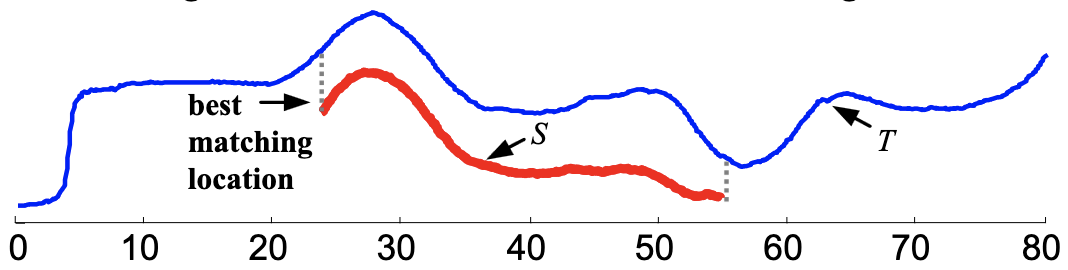
\includegraphics[width=0.5\linewidth]{img/subsequencedist.png}
    \caption{The best matching location of $S$ over $T$.}
    \label{fig:subseq-dist}
\end{figure}

\subsubsection{Shapelet Extraction}

The simplest way to extract shapelets is the \textbf{brute-force approach}, which generates all subsequences of all lengths from the time series in the dataset and adds them to the pool of candidates. Assume each series carries one of two possible class labels. For every candidate, the algorithm checks how well it separates the objects of one class from the other and keeps the best performer. First the series are ordered by their distance from the current candidate; then the split point that maximizes the \textbf{information gain} is found, much as splits are chosen in Decision Tree training. After the information gain of every candidate is computed, the one with the highest value wins.

A common measure used to evaluate information gain is entropy:
\begin{equation*}
    I(D) = -p(A) \log_2 (p(A)) -p(B) \log_2 (p(B)) \,,
\end{equation*}
where $p(A)$ and $p(B)$ are the proportions of objects in classes $A$ and $B$, the two classes making up the time-series dataset $D$. Given a rule that splits $D$ into two subsets $D_1$ and $D_2$, the information remaining after the split is the weighted average entropy of the subsets. Writing $f(D_1)$ and $f(D_2)$ for the fractions of objects in $D_1$ and $D_2$, the total entropy after the split is:
\begin{equation*}
    \hat{I}(D) = f(D_1)I(D_1) + f(D_2)I(D_2)
\end{equation*}
The information gain for a splitting rule is given by the difference of the entropy before and after the split:
\begin{equation*}
    \textit{Gain}(\textit{split}) = I(D) - \hat{I}(D) =  I(D) - f(D_1)I(D_1) - f(D_2)I(D_2)
\end{equation*}

We use the distance from a series $T$ to a shapelet $S$ as the splitting rule $sp$. The total number of candidates generated by the brute-force approach amounts to:
\begin{equation*}
    \sum_{l = \textit{minlen}}^{\textit{maxlen}} \sum_{T_i \in D}(|T_i| - l + 1)
\end{equation*}
For each of these candidates, the distance to every training series must be computed, along with the entropy of each split. This is highly inefficient in both space and time. Two speedups help:
\begin{itemize}
    \item \textbf{Distance early abandon}: cut the time to compute the distance between two series. In the brute-force approach, the distance between a series $T$ and a subsequence $S$ is the minimum Euclidean distance between $S$ and each subsequence of length $|S|$ in $T$, and this costs $O(|T| \cdot |S|)$: there are $O(|T|)$ candidate positions, each Euclidean distance costing $O(|S|)$. But the only distance we keep is the minimum. Rather than compute them all, we stop once the running distance starts to exceed the smallest value seen so far. This is the early-abandon technique.

    \item \textbf{Admissible entropy pruning}: cut the number of distance computations. We only want the best shapelet per class. The most expensive step is computing the distance between a candidate and its nearest matching subsequence in each series of the dataset. Instead of waiting for all those distances, we compute an upper bound on the information gain from the distances known so far. As soon as this upper bound cannot beat the best gain found so far, we stop the distance computations and prune the candidate, since it can never win. The bound comes from comparing the best candidate's information gain against the current candidate's, assuming that every training instance not yet compared is classified perfectly.
\end{itemize}

Another way to extract shapelets is the \textbf{gradient-based method}. The minimum distances $M$ between series and shapelets serve as predictors to approximate the series labels $Y$ through a linear model $W$:
\begin{equation*}
    \hat{Y}_i = W_0 + \sum_{k=1}^KM_{i,k}W_k \;\;\; \forall i \in \{1,..,l\}
\end{equation*}
A logistic regression loss can measure the quality of the prediction:
\begin{equation*}
    L(Y,\hat{Y}) = -Y\ln \sigma (\hat{Y})-(1-Y)\ln(1-\sigma(\hat{Y}))
\end{equation*}
The objective is to minimize a regularized loss function across all the instances (I):
\begin{equation*}
   argmin_{S,W}\,\, F(S,W) = argmin_{S,W}\,\, \sum_{i=1}^l L(Y_i,\hat{Y}_i) + \lambda_W||W||^2
\end{equation*}
We can find the optimal shapelet for the objective in a neural-network fashion, updating the shapelets along the descent direction of the objective, that is, the negative gradient. The weights are updated jointly toward the same minimum.
\paragraph{Shapelets Summary}
\begin{enumerate}
 \item Extract all possible subsequences of a set given lengths (candidate shapelets)
 \item For each candidate shapelet
\begin{enumerate}
    \item Calculate the distance with each time series keeping the minimum distance (best alignment)
    \item Evaluate the discriminatory effect of the shapelet through the Information Gain
\end{enumerate}
 \item  Return the k best shapelets with the
highest Information Gain.
    \item  Transform a dataset and train a ML model.
\end{enumerate}